%
%----------------------------------------------------------------------------------------
%	PACKAGES AND DOCUMENT CONFIGURATIONS
%----------------------------------------------------------------------------------------
%

\documentclass[12pt]{article} %report, article, amsart, exam
\usepackage[letterpaper,margin=1in]{geometry}
\usepackage{fancyhdr,color}
\usepackage{tikz,graphicx,multicol}
\usepackage{amssymb,euscript,eufrak,nicefrac,enumitem}
\usepackage{amsfonts,amsmath,amsthm} %don't need with 'amsart' document class
\usepackage{hyperref}
\usepackage{comment}
\usepackage{scrextend} %needed for addmargin environment
\usepackage{graphicx} 
\usepackage{listings}

\usepackage{color}
\usepackage{accsupp}
\usepackage{booktabs}
\usepackage{subcaption}

\definecolor{dkblue}{rgb}{0,0,0.5}
\definecolor{comment}{rgb}{1,0,0}
\definecolor{mauve}{rgb}{.627,.126,.941}
\definecolor{purple}{rgb}{0.5, 0, 0.545098}

\lstdefinestyle{customc}{
  belowcaptionskip=1\baselineskip,
  breaklines=true,
  frame=L,
  xleftmargin=\parindent,
  language=C,
  showstringspaces=false,
  basicstyle=\footnotesize\ttfamily,
  keywordstyle=\bfseries\color{green!40!black},
  commentstyle=\itshape\color{purple!40!black},
  identifierstyle=\color{blue},
  stringstyle=\color{orange},
}

\lstdefinestyle{customasm}{
  belowcaptionskip=1\baselineskip,
  frame=L,
  xleftmargin=\parindent,
  language=[x86masm]Assembler,
  basicstyle=\footnotesize\ttfamily,
  commentstyle=\itshape\color{purple!40!black},
}

\lstset{escapechar=@,style=customc}

%
%----------------------------------------------------------------------------------------
%% Define headers & footers
%----------------------------------------------------------------------------------------

\pagestyle{fancy}
   \lhead{} 
   %\chead{Loyola University Chicago} 
   \rhead{}
   \renewcommand{\headrulewidth}{0pt}
   \addtolength{\footnotesep}{5mm}
 
%
%----------------------------------------------------------------------------------------
%% Some user-defined colors
%----------------------------------------------------------------

\setlength{\parskip}{1em}
\renewcommand{\baselinestretch}{1.3}

%
%----------------------------------------------------------------------------------------
%% BEGIN: topmatter
%----------------------------------------------------------------------------------------
%

\title{ COMP 464 - High Performance Computing \\ OpenMP Threading} % Title
\author{
Loyola University Chicago \\
Jose Luis Rodriguez 
} % Author name
\date{\today} % Date for the report

%
%% END: topmatter
%%------------------------------

\begin{document}

\maketitle

\thispagestyle{fancy}

%---------------------------------------------------------------------------------------- 
%	SECTION 1 - PROBLEM STATEMENT
%----------------------------------------------------------------------------------------

\section{Overview}

This report highlights the procedures and results of running the nbody3 C++ code that predicts the individual motion of a group of celestial objects (particles) interacting with each other gravitationally. The program also runs a series of experiments and generates a benchmark (max, min and average speed) utilizing the Stampede2 supercomputer at The University of Texas at Austin?s Texas Advanced Computing Center (TACC). The nbody3 code utilize Intel C++ library compilers and the OpenMP library in order to parallelize the serial code details and speci?cations to follow.

The n-body problem code performs two major benchmarks in order to compute strong scalability and weak scalability. The program was compiled in serial and parallel each version was tested with 1,000, 2,000, 4,000, and 8,000 particles and 1, 2, 4, 8, 16, 32, and 64 threads, all tests ran with the same number of steps (-s 500). The average time per number of particles was recored in order to compute the strong scalability. This method also allows to compute the weak scalability test as we are keeping a constant workload per-thread when the number of particles increase the number of threads also increased. To ?nd out the number of particles needed per thread the parallel code was executed keeping the number of particles and steps constant (n=1000, s=200) while increasing the number of threats.

\section{Benchmark Analysis}

\textbf{Code Mofications} 

In order to perform the benchmarks in parallel, pragmas ( statements tell the compiler to use the OpenMP framework to parallelize the code) were used on the outer for loops of the accelerate, update and search functions. In the later also a reduction on the min, max and average velocity was used, snippets of the code can be found in the reference.

\subsection{Strong scalability}
When the nbody problem particles size stays ?xed or increased as the number of processing elements are increased. In Figure.1 Stampede2 compute node using the GNU compiler, we can see how the benchmark that uses most bandwidth is the \textsc{COPY} benchmark, with a top performance at $26kb$

\begin{figure}[htb]
\caption{Strong Scaling - Speed-Up (T1/Tp)}\label{fig:benchmark01}
\centering
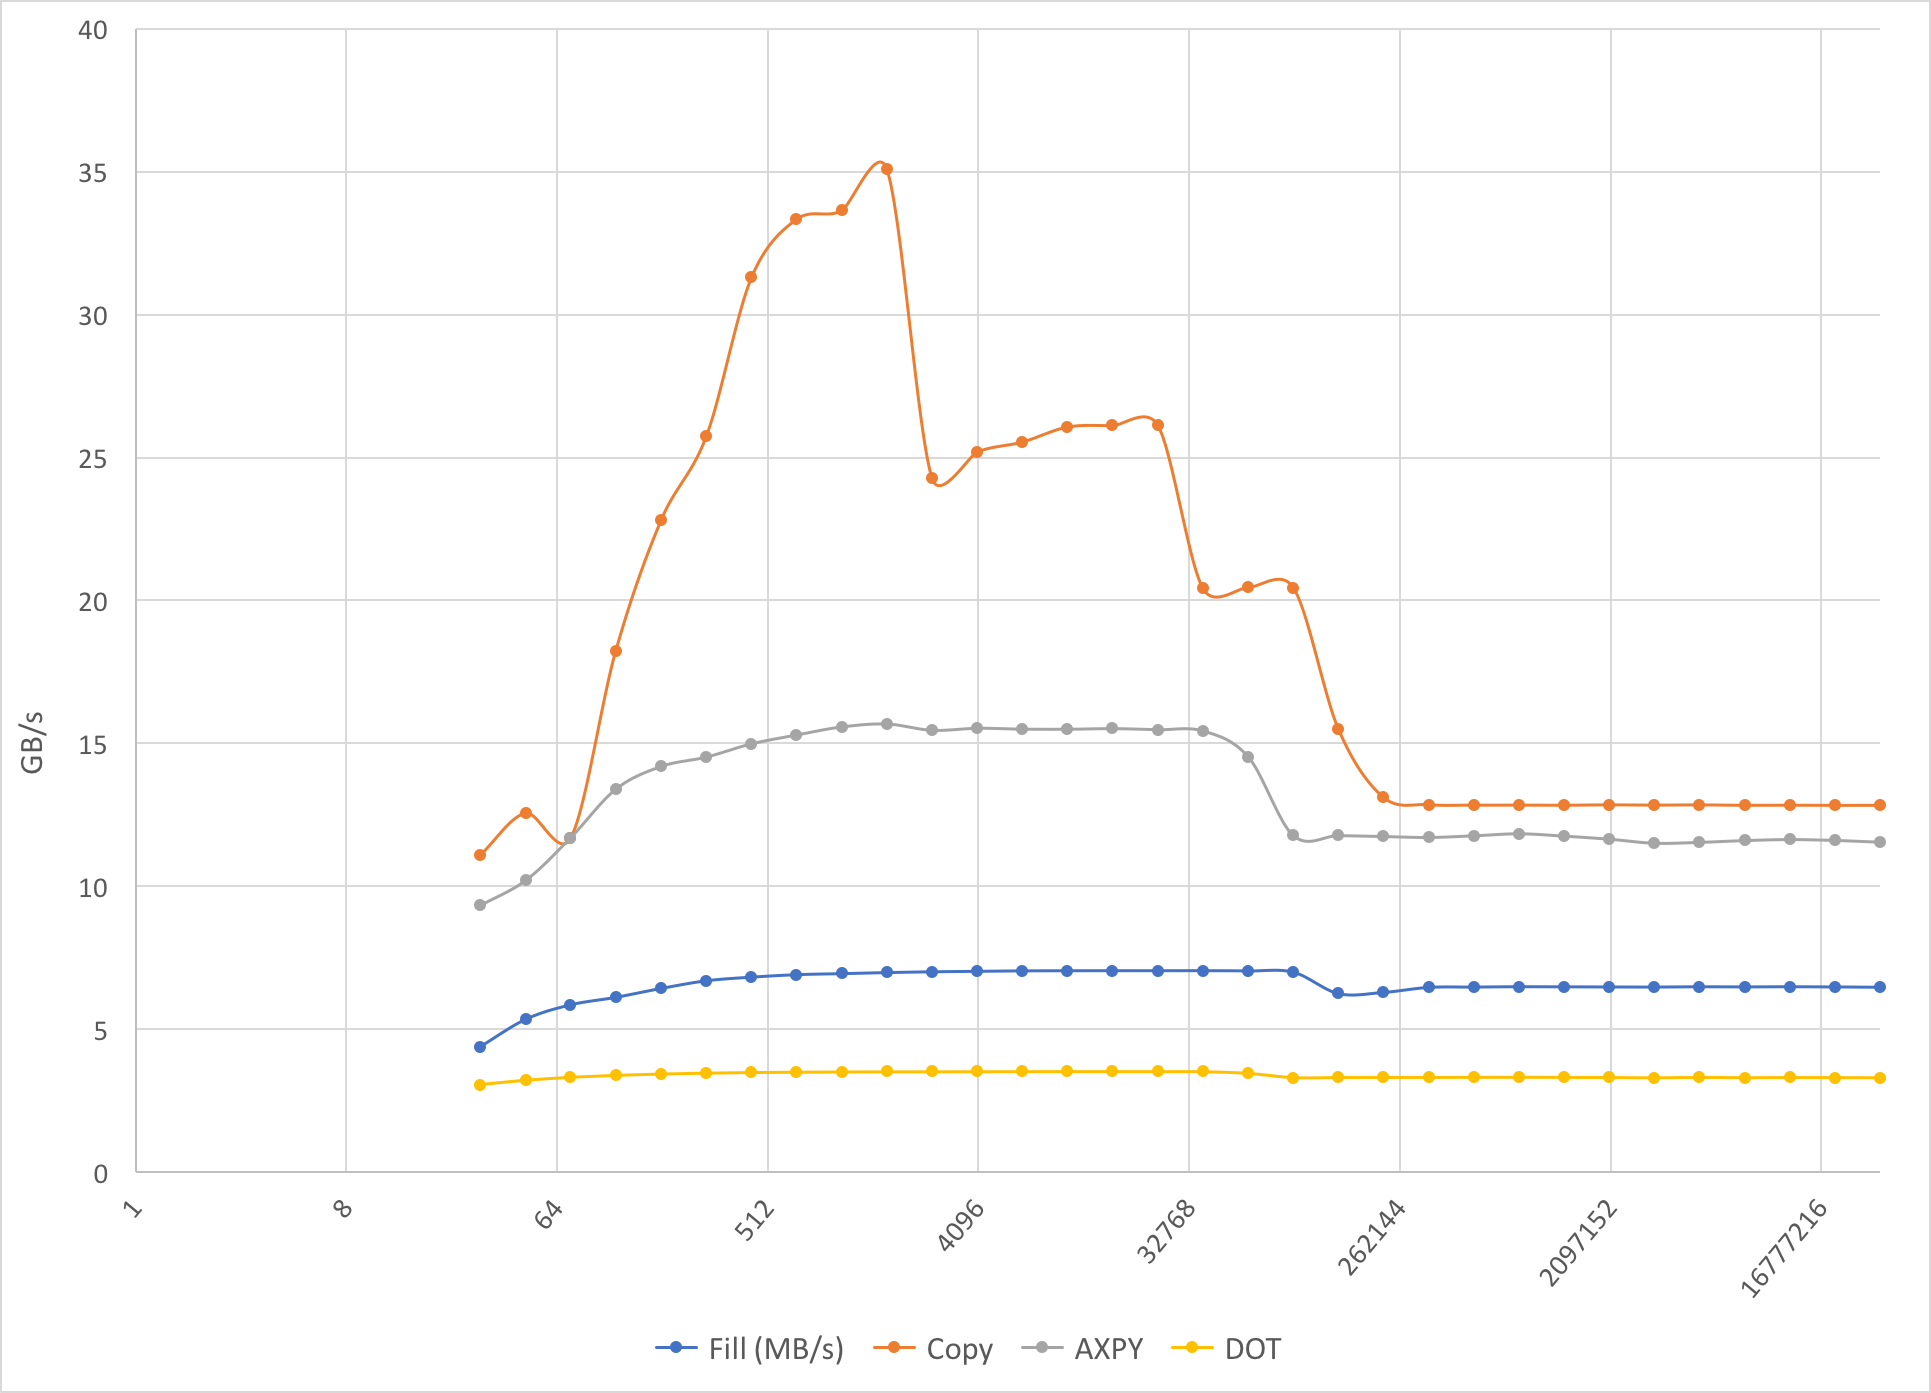
\includegraphics[width=\textwidth,keepaspectratio]{imgs/img01.png}
\end{figure} 


\newpage

In Figure.1 Stampede2 compute node using the GNU compiler, we can see how the benchmark that uses most bandwidth is the \textsc{COPY} benchmark, with a top performance at $26kb$ right before filling the $32kb$ L1 cache then we see another drop at approximately after 534kb array size when L2 cache gets  filled. The other benchmarks seem to behave more or less similarly, some of them show some drops but nothing close to what the \textsc{COPY} benchmark experience.

\begin{figure}[htb]
\caption{Strong Scaling - Efficiency (Sp/P)}\label{fig:benchmark01}
\centering
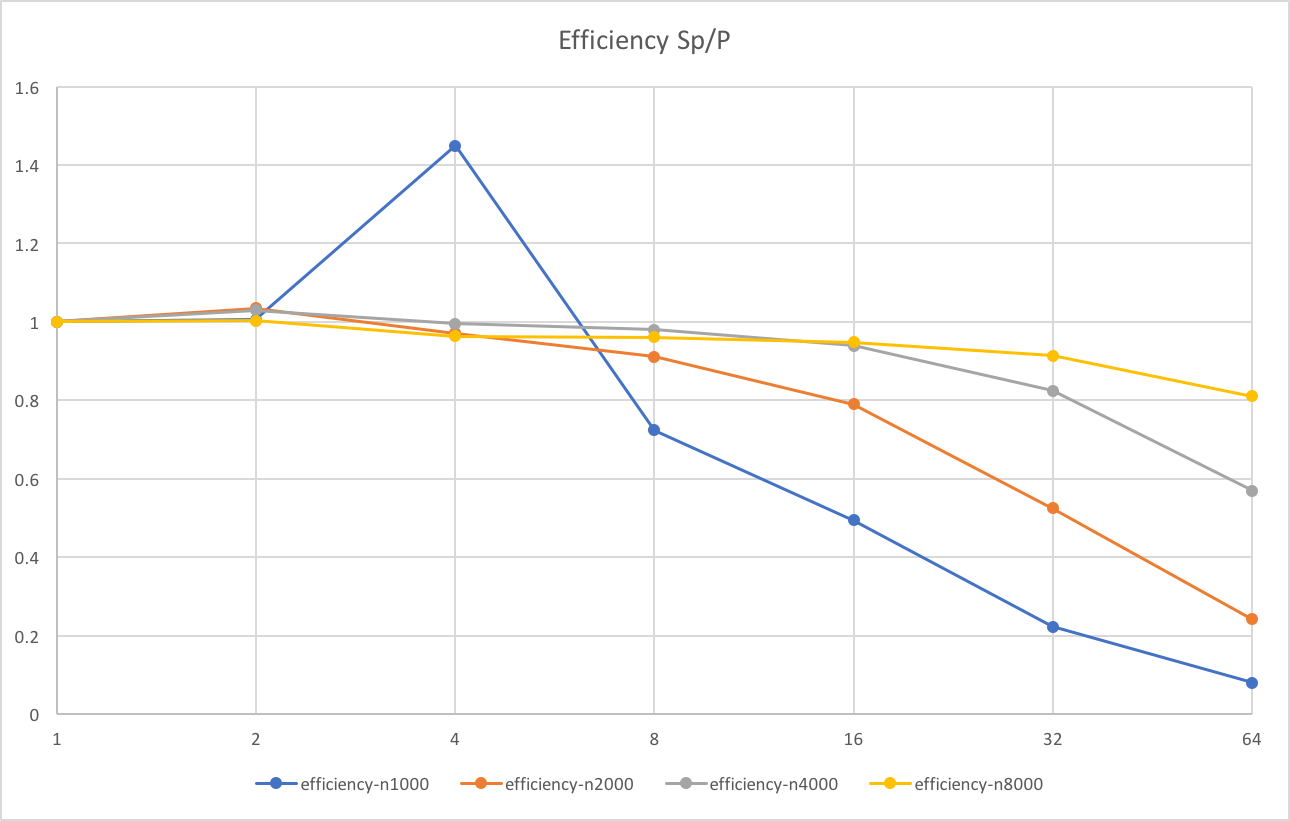
\includegraphics[width=\textwidth,keepaspectratio]{imgs/img02.png}
\end{figure} 

\newpage

\subsection{Weak scalability}

When the nbody problem size particles assigned to each processing element stays constant and additional elements are used to solve the nbbody problem. Now in Figure.2 we change the compiler to Intel's C++ compiler and we can see significant changes on all the benchmarks. The most prominent change from the previous figure is the \textsc{AXPY}  

benchmark that peeks approximately around $40kb$ with a much higher bandwidth almost 120 times higher compared with the GNU compiler.  The \textsc{FILL} benchmark also shows signs of a significant drop with a peek at 32kb and $100$Gb\/s to $40$Gb\/s  after the $L1$ gets filled.

\begin{figure}[htb]
\caption{Weak Scaling - Speed-Up (T1/Tp)}\label{fig:benchmark02}
\centering
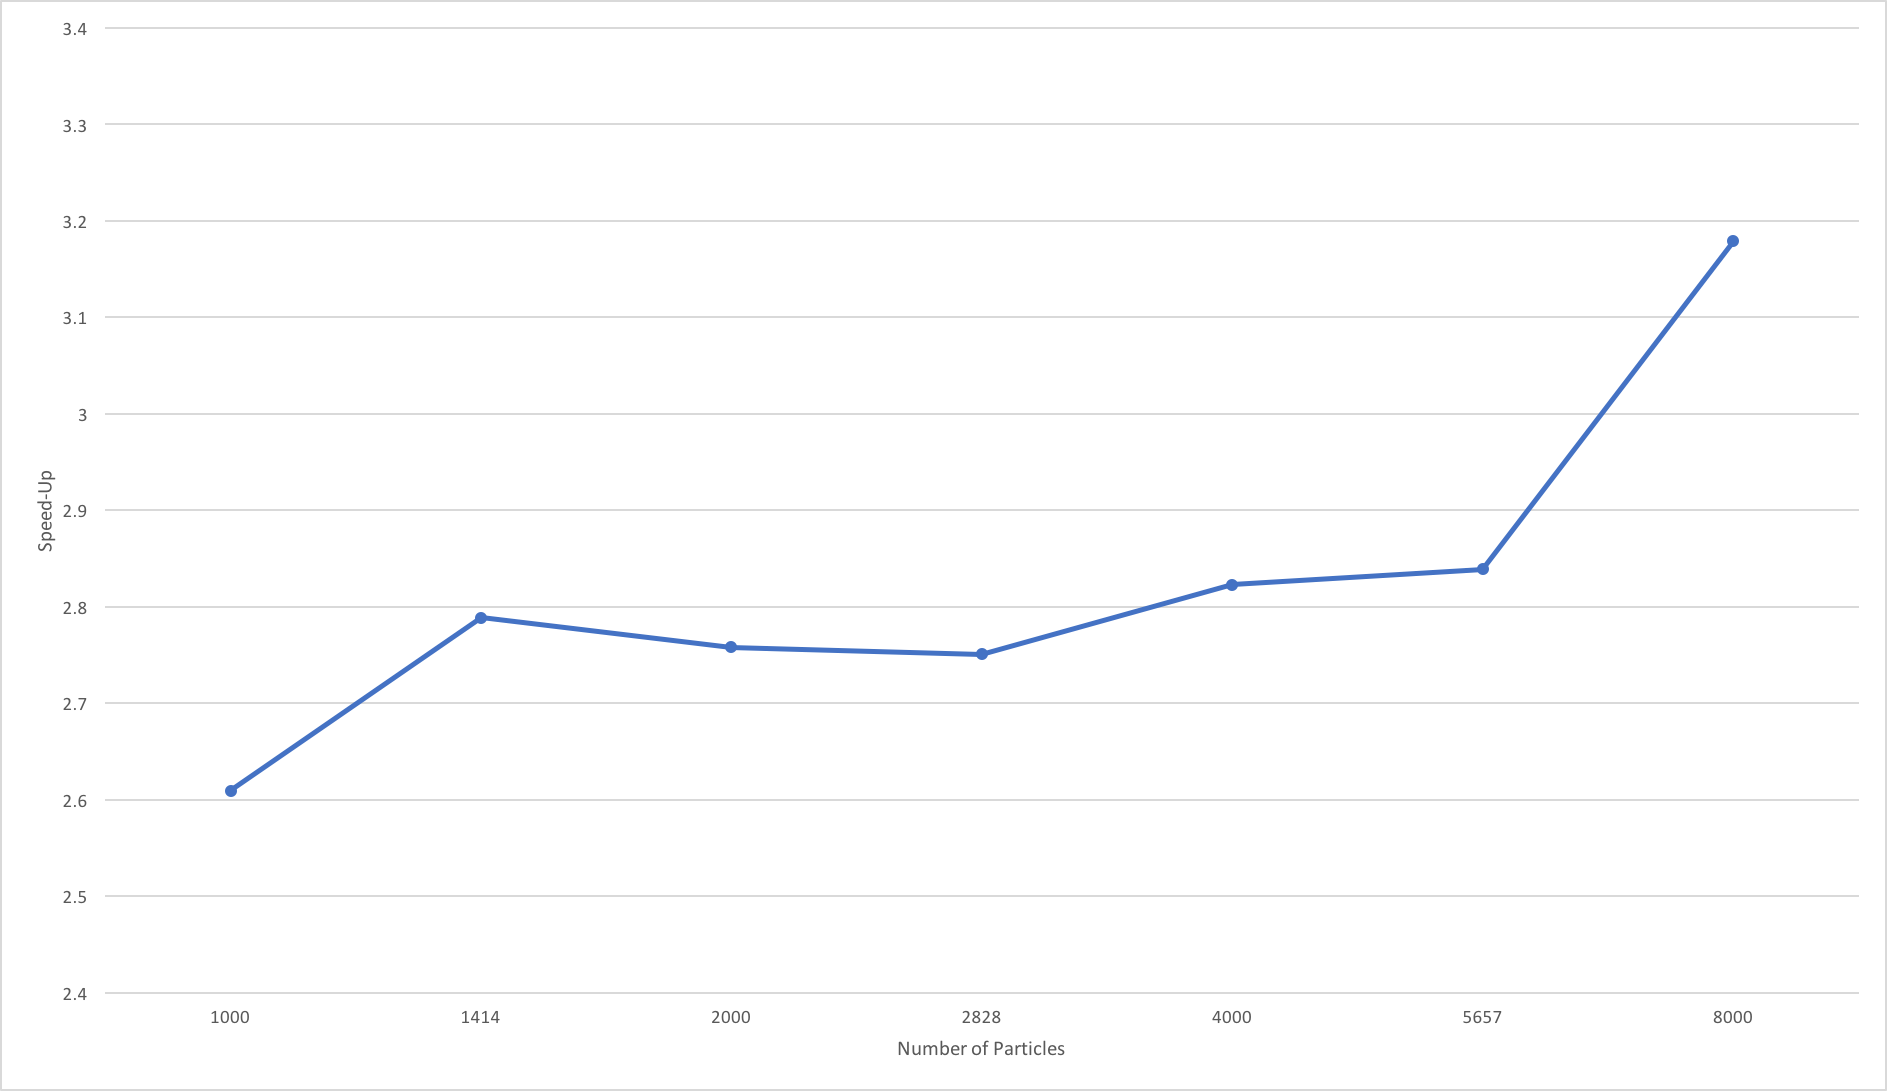
\includegraphics[width=\textwidth,keepaspectratio]{imgs/img03.png}
\end{figure}

\newpage

Now in Figure.2 we change the compiler to Intel's C++ compiler and we can see significant changes on all the benchmarks. The most prominent change from the previous figure is the \textsc{AXPY}  benchmark that peeks approximately around $40kb$ with a much higher bandwidth almost 120 times higher compared with the GNU compiler.  The \textsc{FILL} benchmark also shows signs of a significant drop with a peek at 32kb and $100$Gb\/s to $40$Gb\/s  after the $L1$ gets filled.

\begin{figure}[htb]
\caption{Weak Scaling - Efficiency (Sp/P)}\label{fig:benchmark02}
\centering
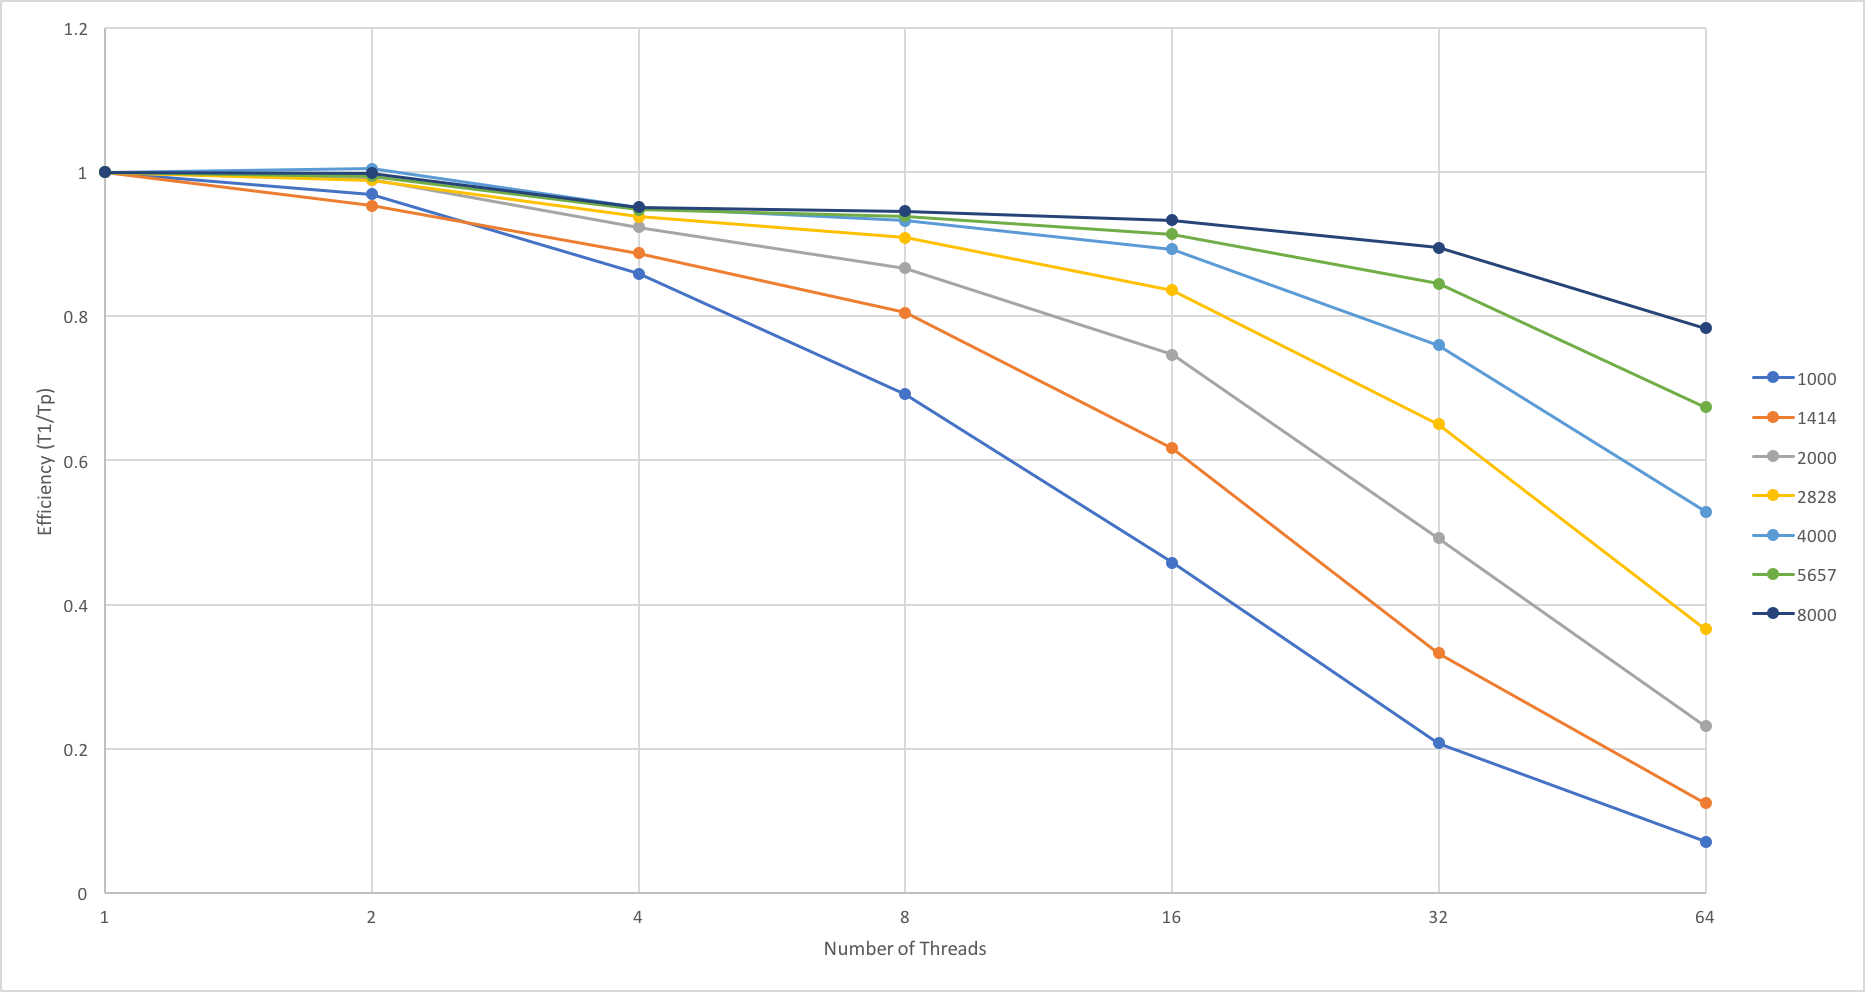
\includegraphics[width=\textwidth,keepaspectratio]{imgs/img04.png}
\end{figure}


%----------------------------------------------------------------
%	SECTION 3 - REFERENCE
%----------------------------------------------------------------

\section{Reference}

\begin{flushleft}
Stampede2 User Guide -- Managing Memory \\ \url{https://portal.tacc.utexas.edu/user-guides/stampede2#managingmemory}

Introduction to High Performance Scientific Computing -- Victor Eijkhout \\ \url{http://pages.tacc.utexas.edu/~eijkhout/istc/istc.html}
\end{flushleft}

\newpage


\begin{table}[]
\centering
\caption{Strong Scaling Benchmark - Number of Particles: 1000}
\resizebox{\textwidth}{!}{%
\begin{tabular}{@{}cccc@{}}
\toprule
\textbf{Threads} & \textbf{runtime-n1000} & \textbf{speed-up-n1000} & \textbf{efficiency-n1000} \\ \midrule
1 & 2.699547 & 1.00 & 1.00 \\
2 & 1.342266 & 2.01 & 1.01 \\
4 & 0.767273 & 3.52 & 0.88 \\
8 & 0.465877 & 5.79 & 0.72 \\
16 & 0.340848 & 7.92 & 0.50 \\
32 & 0.378338 & 7.14 & 0.22 \\
64 & 0.527209 & 5.12 & 0.08 \\ \bottomrule
\end{tabular}%
}
\end{table}

\begin{table}[]
\centering
\caption{Strong Scaling Benchmark - Number of Particles: 2000}
\resizebox{\textwidth}{!}{%
\begin{tabular}{@{}cccc@{}}
\toprule
\textbf{Threads} & \textbf{runtime-n2000} & \textbf{speed-up-n2000} & \textbf{efficiency-n2000} \\ \midrule
1 & 10.702174 & 1.00 & 1.00 \\
2 & 5.170901 & 2.07 & 1.03 \\
4 & 2.755932 & 3.88 & 0.97 \\
8 & 1.468389 & 7.29 & 0.91 \\
16 & 0.846486 & 12.64 & 0.79 \\
32 & 0.636906 & 16.80 & 0.53 \\
64 & 0.689989 & 15.51 & 0.24 \\ \bottomrule
\end{tabular}%
}
\end{table}

\begin{table}[]
\centering
\caption{Strong Scaling Benchmark - Number of Particles: 4000}
\resizebox{\textwidth}{!}{%
\begin{tabular}{@{}cccc@{}}
\toprule
\textbf{Threads} & \textbf{runtime-n4000} & \textbf{speed-up-n4000} & \textbf{efficiency-n4000} \\ \midrule
1 & 42.174895 & 1.00 & 1.00 \\
2 & 20.477445 & 2.06 & 1.03 \\
4 & 10.593958 & 3.98 & 1.00 \\
8 & 5.375854 & 7.85 & 0.98 \\
16 & 2.804787 & 15.04 & 0.94 \\
32 & 1.598818 & 26.38 & 0.82 \\
64 & 1.155382 & 36.50 & 0.57 \\ \bottomrule
\end{tabular}%
}
\end{table}

\begin{table}[]
\centering
\caption{Strong Scaling Benchmark - Number of Particles: 8000}
\resizebox{\textwidth}{!}{%
\begin{tabular}{@{}cccc@{}}
\toprule
\textbf{Threads} & \textbf{runtime-n8000} & \textbf{speed-up-n8000} & \textbf{efficiency-n8000} \\ \midrule
1 & 161.399121 & 1.00 & 1.00 \\
2 & 80.410162 & 2.01 & 1.00 \\
4 & 41.872722 & 3.85 & 0.96 \\
8 & 21.005236 & 7.68 & 0.96 \\
16 & 10.634796 & 15.18 & 0.95 \\
32 & 5.517657 & 29.25 & 0.91 \\
64 & 3.109065 & 51.91 & 0.81 \\ \bottomrule
\end{tabular}%
}
\end{table}

\begin{table}[]
\centering
\caption{Weak Scaling Benchmark - Number of Particles: 1000}
\resizebox{\textwidth}{!}{%
\begin{tabular}{@{}cccc@{}}
\toprule
\textbf{Threads} & \textbf{runtime-n1000} & \textbf{speed-up-n1000} & \textbf{efficiency-n1000} \\ \midrule
1 & 2.551973 & 1.00 & 1.00 \\
2 & 1.307288 & 1.95 & 0.98 \\
4 & 0.713981 & 3.57 & 0.89 \\
8 & 0.407256 & 6.27 & 0.78 \\
16 & 0.27913 & 9.14 & 0.57 \\
32 & 0.303005 & 8.42 & 0.26 \\
64 & 0.447266 & 5.71 & 0.09 \\ \bottomrule
\end{tabular}%
}
\end{table}


\begin{table}[]
\centering
\caption{Weak Scaling Benchmark - Number of Particles: 2000}
\resizebox{\textwidth}{!}{%
\begin{tabular}{@{}cccc@{}}
\toprule
\textbf{Threads} & \textbf{runtime-n2000} & \textbf{speed-up-n2000} & \textbf{efficiency-n2000} \\ \midrule
1 & 10.067885 & 1.00 & 1.00 \\
2 & 5.085486 & 1.98 & 0.99 \\
4 & 2.698663 & 3.73 & 0.93 \\
8 & 1.399622 & 7.19 & 0.90 \\
16 & 0.78047 & 12.90 & 0.81 \\
32 & 0.555237 & 18.13 & 0.57 \\
64 & 0.574328 & 17.53 & 0.27 \\ \bottomrule
\end{tabular}%
}
\end{table}

\begin{table}[]
\centering
\caption{Weak Scaling Benchmark - Number of Particles: 4000}
\resizebox{\textwidth}{!}{%
\begin{tabular}{@{}cccc@{}}
\toprule
\textbf{Threads} & \textbf{runtime-n4000} & \textbf{speed-up-n4000} & \textbf{efficiency-n4000} \\ \midrule
1 & 39.98665 & 1.00 & 1.00 \\
2 & 20.032609 & 2.00 & 1.00 \\
4 & 10.537717 & 3.79 & 0.95 \\
8 & 5.324176 & 7.51 & 0.94 \\
16 & 2.753726 & 14.52 & 0.91 \\
32 & 1.53249 & 26.09 & 0.82 \\
64 & 1.075133 & 37.19 & 0.58 \\ \bottomrule
\end{tabular}%
}
\end{table}


\begin{table}[]
\centering
\caption{Weak Scaling Benchmark - Number of Particles: 8000}
\resizebox{\textwidth}{!}{%
\begin{tabular}{@{}cccc@{}}
\toprule
\textbf{Threads} & \textbf{runtime-n8000} & \textbf{speed-up-n8000} & \textbf{efficiency-n8000} \\ \midrule
1 & 158.33655 & 1.00 & 1.00 \\
2 & 79.404148 & 1.99 & 1.00 \\
4 & 41.873768 & 3.78 & 0.95 \\
8 & 20.95203 & 7.56 & 0.94 \\
16 & 10.574536 & 14.97 & 0.94 \\
32 & 5.472768 & 28.93 & 0.90 \\
64 & 3.098319 & 51.10 & 0.80 \\ \bottomrule
\end{tabular}%
}
\end{table}


\begin{figure}[]
\caption{OpenMP Pragmas for Acceleration Function}\label{fig:benchmark01}
\begin{lstlisting}
template <typename ValueType>
void accel_register (	ValueType * __RESTRICT pos, 
			ValueType * __RESTRICT vel, 
			ValueType * __RESTRICT mass, 
			ValueType * __RESTRICT acc, 
			const int n)
{
   #pragma omp parallel
    {
    #pragma omp for
       for (int i = 0; i < n; ++i)
       {
          ValueType ax = 0, ay = 0, az = 0;
          const ValueType xi = pos_array(i,0);
          const ValueType yi = pos_array(i,1);
          const ValueType zi = pos_array(i,2);
          for (int j = 0; j < n; ++j)
          {
             /* Position vector from i to j and the distance^2. */
             ValueType rx = pos_array(j,0) - xi;
             ValueType ry = pos_array(j,1) - yi;
             ValueType rz = pos_array(j,2) - zi;
             ValueType dsq = rx*rx + ry*ry + rz*rz + TINY2;
             ValueType m_invR3 = mass[j] / (dsq * std::sqrt(dsq));
    
             ax += rx * m_invR3;
             ay += ry * m_invR3;
             az += rz * m_invR3;
          }
    
          acc_array(i,0) = G * ax;
          acc_array(i,1) = G * ay;
          acc_array(i,2) = G * az;
       }
    }
}
\end{lstlisting}
\end{figure}

\begin{figure}[]
\caption{OpenMP Pragmas for Update Function}\label{fig:benchmark01}
\begin{lstlisting}
template <typename ValueType>
void update (ValueType pos[], ValueType vel[], ValueType mass[], ValueType acc[], const int n, ValueType h)
{
    #pragma omp parallel
    {
    #pragma omp for
       for (int i = 0; i < n; ++i)
          for (int k = 0; k < NDIM; ++k)
          {
             pos_array(i,k) += vel_array(i,k)*h + acc_array(i,k)*h*h/2;
             vel_array(i,k) += acc_array(i,k)*h;
          }
    }
}
\end{lstlisting}
\end{figure}

\begin{figure}[]
\caption{OpenMP Pragmas for Search Function}\label{fig:benchmark01}
\begin{lstlisting}
template <typename ValueType>
void search (ValueType pos[], ValueType vel[], ValueType mass[], ValueType acc[], const int n)
{
  ValueType minv = 1e10, maxv = 0, ave = 0;
  #pragma omp parallel default(none) shared(minv,maxv,ave)
  {
  #pragma omp for reduction(+:ave) reduction(max:maxc) reduction(min:minv)       
   for (int i = 0; i < n; ++i)
   {
         ValueType vmag = 0;
         for (int k = 0; k < NDIM; ++k)
         	vmag += (vel_array(i,k) * vel_array(i,k));
         vmag = sqrt(vmag);
         maxv = std::max(maxv, vmag);
         minv = std::min(minv, vmag);
         ave += vmag;
    }
   printf("min/max/ave velocity = %e, %e, %e\n", minv, maxv, ave/n);
  }
}
\end{lstlisting}
\end{figure}

\begin{table}[]
\centering
\caption{Stampede2 - Compute Node (knl) - System Information}
\resizebox{\textwidth}{!}{%
\begin{tabular}{@{}ll@{}}
\toprule
\textbf{Architecture} & x86\_64 \\ \midrule
\textbf{CPU op-mode(s)} & 32-bit, 64-bit \\
\textbf{Byte Order} & Little Endian \\
\textbf{CPU(s)} & 272 \\
\textbf{On-line CPU(s) list} & 0-271 \\
\textbf{Thread(s) per core} & 4 \\
\textbf{Core(s) per socket} & 68 \\
\textbf{Socket(s)} & 1 \\
\textbf{NUMA node(s)} & 2 \\
\textbf{Vendor ID} & GenuineIntel \\
\textbf{CPU family} & 6 \\
\textbf{Model} & 87 \\
\textbf{Model name} & Intel(R) Xeon Phi(TM) CPU 7250 @ 1.40GHz \\
\textbf{Stepping} & 1 \\
\textbf{CPU MHz} & 1255.132 \\
\textbf{BogoMIPS} & 2793.44 \\
\textbf{L1d cache} & 32K \\
\textbf{L1i cache} & 32K \\
\textbf{L2 cache} & 1024K \\
\textbf{NUMA node0 CPU(s)} & 0-271 \\
\textbf{NUMA node1 CPU(s)} &  \\ \bottomrule
\end{tabular}%
}
\end{table}


\end{document}